\section{Evaluation}
In this section, we compare several LSH methods: basic LSH, LSH forest and multi-probe LSH.
We conduct experiments with parameters show in \cref{tbl:exp-settings}.

\begin{table}
\centering
  \caption{Experiment Settings}
  \begin{tabular}{cccc}
		\hline
		Algorithm & Basic & LSHForest & MultiProbe  \\ \hline
		\#compounds & 8 & 25 & 8 \\\hline
		$w$ & 8 & 1 & 8 \\\hline
	\end{tabular}
	\label{tbl:exp-settings}
\end{table}
\subsection{Datasets}
We use MNIST \footnote{http://yann.lecun.com/exdb/mnist/} to evaluate LSH methods. MNIST contains 60000 28$\times$28 images in training set, and 10000 images in testing set.
We select 50 dimension out of the 28$\times$28 dimensions with largest variances as features.
We select 100 images from the testing set as testing samples.
Then we use linear scan to get the ground truth.
\subsection{Evaluation Metrics}
Error ratio evaluate how close the candidates found by LSH is to ground truth objects.
Recall shows how many nearest neighbors are found by LSH.
$$
\text{Error Ratio}=\frac{1}{N}\frac{1}{K}\sum_{n=1}^{N}\sum_{i=1}^{K}\frac{d(q, p_{lsh}^{(i)})}{d(q, p_{label}^{(i)})}, \>\>\>\>
\text{Recall}=\frac{|A_{lsh}\cap A_{label}|}{|A_{label}|}
$$
We also use hash table building time and query time to evaluate the efficiency. Since the query is also highly dependent on the number of candidates, we also present $c/n=\frac{\#candiate}{\#all train samples}$.

\subsection{Effectiveness}

\begin{figure*}[hbt]
\label{fig:effectiveness}
\begin{subfigure}{\columnwidth}
  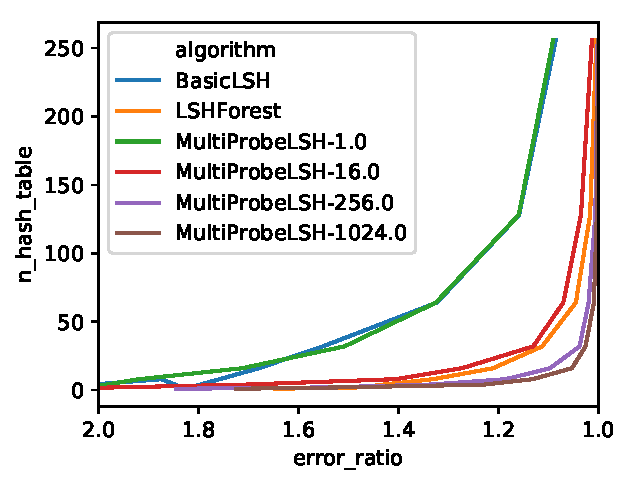
\includegraphics[width=\columnwidth]{figures/error_ratio}
\end{subfigure}
\begin{subfigure}{\columnwidth}
  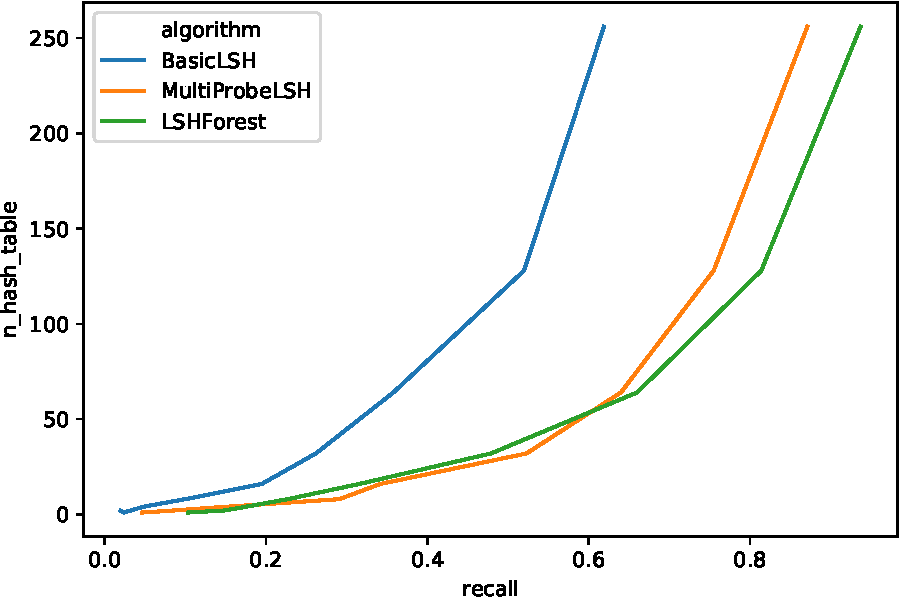
\includegraphics[width=\columnwidth]{figures/recall}
\end{subfigure}
\caption{Error ratio and recall comparison.}
\end{figure*}

The results are presented in \cref{fig:effectiveness}.
We present results of multi-probe LSH with different numbers of probe $T$.
When $T=1$, multi-probe LSH is exactly the same with basic LSH.
As $T$ increases, multi-probe LSH achieve the same error ratio and recall with less hash tables.
LSH forest achieves similar performance with multi-probe LSH when $T=16$.
Multi-probe LSH can significantly reduce the number of hash table that needed.


\subsection{Time Efficiency}

\begin{figure*}[hbt]
\label{fig:efficiency}
\begin{subfigure}{\columnwidth}
  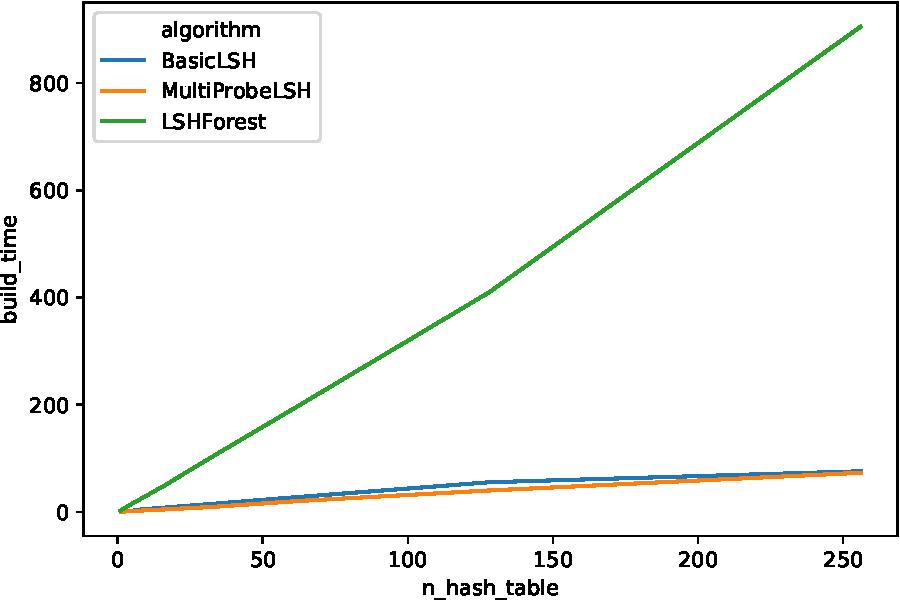
\includegraphics[width=\columnwidth]{figures/build_time}
\end{subfigure}
\begin{subfigure}{\columnwidth}
  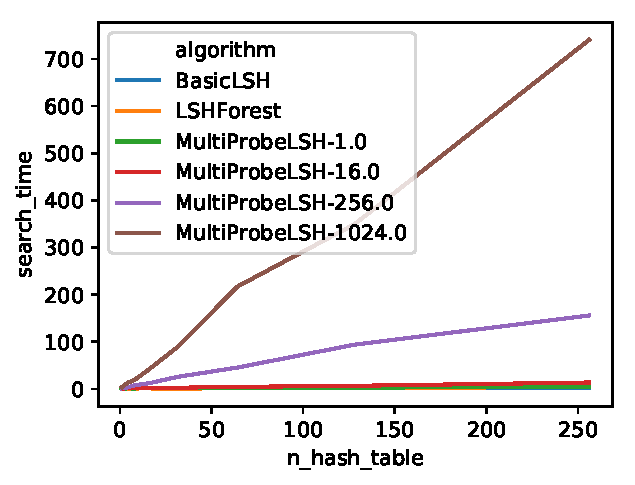
\includegraphics[width=\columnwidth]{figures/search_time}
\end{subfigure}
\begin{subfigure}{\columnwidth}
  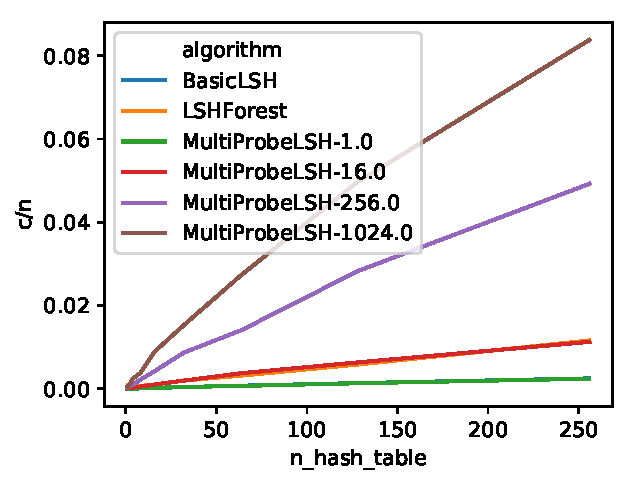
\includegraphics[width=\columnwidth]{figures/c_n}
\end{subfigure}
\begin{subfigure}{\columnwidth}
  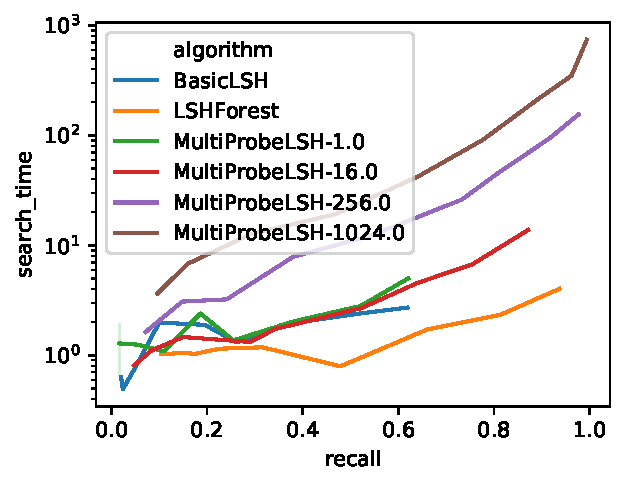
\includegraphics[width=\columnwidth]{figures/recall_search_time}
\end{subfigure}
\caption{Time efficiency comparison.}
\end{figure*}

The results are presented in \cref{fig:efficiency}.
LSH forest consumes much more build time than others.
Actually multi-probe LSH is the same as basic LSH when building.

As $T$ increases, multi-probe LSH return more and more candidates with the same number hash tables.
However, when achieving the same recall, LSH forest still require less search time.








